\chapter{Projekt systemu}
\thispagestyle{chapterBeginStyle}

Niniejszy rozdział traktuje o procesach systemu, jego składowych i powiązaniach między nimi. Do ich przedstawienia używane są opisy słowne oraz diagramy UML. Istotnym elementem jest prezentacja sposobu, w jaki przetwarzane są obrazy w systemie oraz algorytmów z tym związanych.

\section{Przypadki użycia}
Powiązany z systemem jest obecnie jeden, główny przypadek użycia. Aktorem jest gracz, który po uruchomieniu aplikacji mobilnej łączy się z systemem wbudowanym podłączonym do tarczy. Po informacji o ustanowieniu połączenia, może on zacząć wykonywać rzuty. Po każdym rzucie, w krótkim czasie, otrzymuje on informację o polu, w jakie trafił oraz wizualizację miejsca wbicia lotki na graficznym schemacie tarczy. Aplikacja, w razie potrzeby, sygnalizuje problemy z połączeniem na linii klient-serwer.

\section{Urządzenia i komponenty}
W systemie występują następujące urządzenia:
\begin{itemize}
  \item minikomputer \verb|Raspberry Pi 4 B|;
  \item minikomputer \verb|Raspberry Pi Zero W|;
  \item dwie kamery \verb|Camera Module v1 (OmniVision OV5647)|;
  \item smartfon.
\end{itemize}

Na diagramie wdrożenia (\ref{deployment}) pokazano te urządzenia wraz z połączeniami między nimi oraz komponentami, jakie wchodzą w ich skład. \verb|Raspberry Pi 4| jest najważniejszym urządzeniem, które synchronizuje pracę innych oraz dokonuje obliczeń. Łączy się z kamerą za pomocą kabla taśmowego, a używa jej do wykrywania rzutu za pomocą biblioteki \verb|OpenCV|. Analogicznie wygląda to w przypadku \verb|Pi Zero|, na którym znajduje się druga instancja detektora rzutu. Informacje wysyłane są z \verb|Pi Zero| do \verb|Pi 4| z użyciem gniazd TCP. Na \verb|Pi 4| tworzony jest również serwer dla aplikacji mobilnej, która uruchamiana jest na smartfonie w środowisku Expo \cite{expo}. Połączenie następuje zgodnie ze standardem WebSocket.

% TODO: może inna czcionka w UML?
\begin{figure}[h!]
\begin{center}
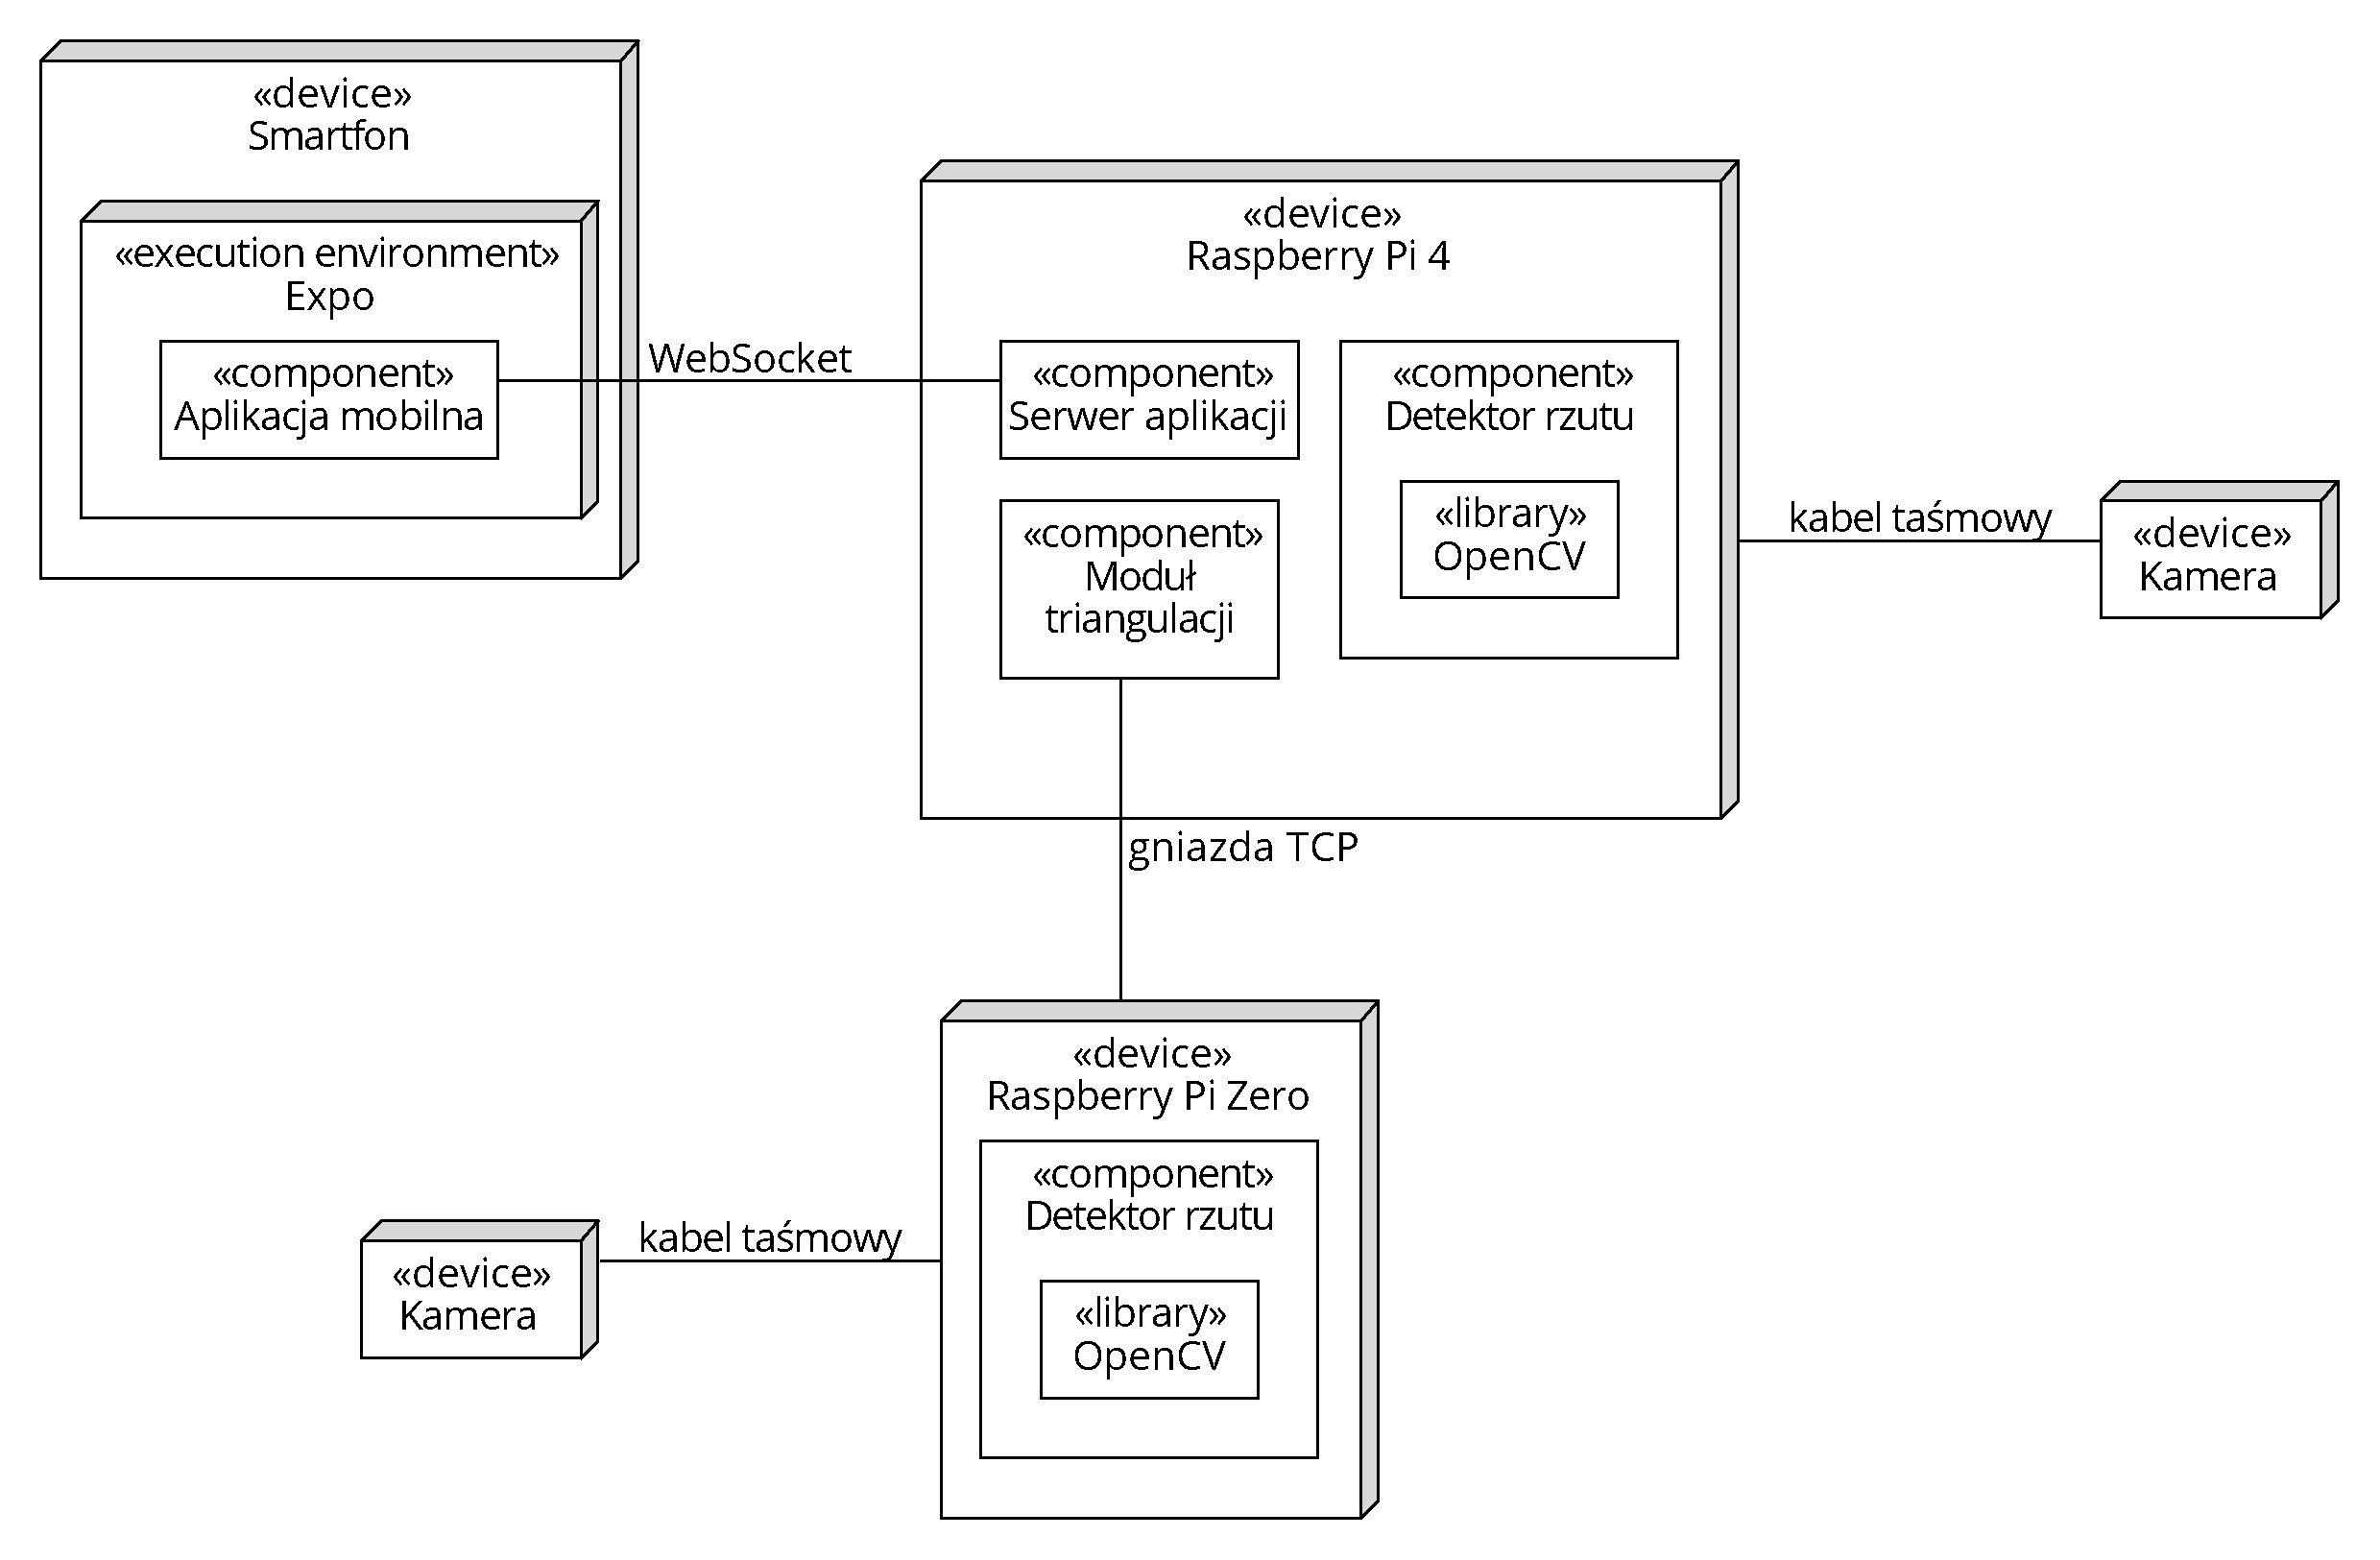
\includegraphics[width=\textwidth]{obrazki/deployment.pdf}
\end{center}
\captionsource{{\color{dgray}Diagram wdrożeniowy}}{Opracowanie własne}
\label{deployment}
\end{figure}

\section{Diagramy aktywności}
Na diagramie aktywności (\ref{activity}) przedstawiono logikę procesu zachodzącego w systemie z zachowaniem wysokiego poziomu ogólności. System rozpoczyna działanie od rozwidlenia na przetwarzanie obrazu z użyciem kamery dolnej oraz prawej. W obu przypadkach wygląda to identycznie - w pętli wykonywane są zdjęcia i poddawane analizie. W przypadku wykrycia rzutu pętla zostaje przerwana, a program synchronizuje się z drugą kamerą i przeprowadza obliczenia prowadzące do pozycji rzutki, która zostaje wyświetlona w aplikacji mobilnej. Następnie proces rozpoczyna się od początku.

\begin{figure}[h!]
\begin{center}
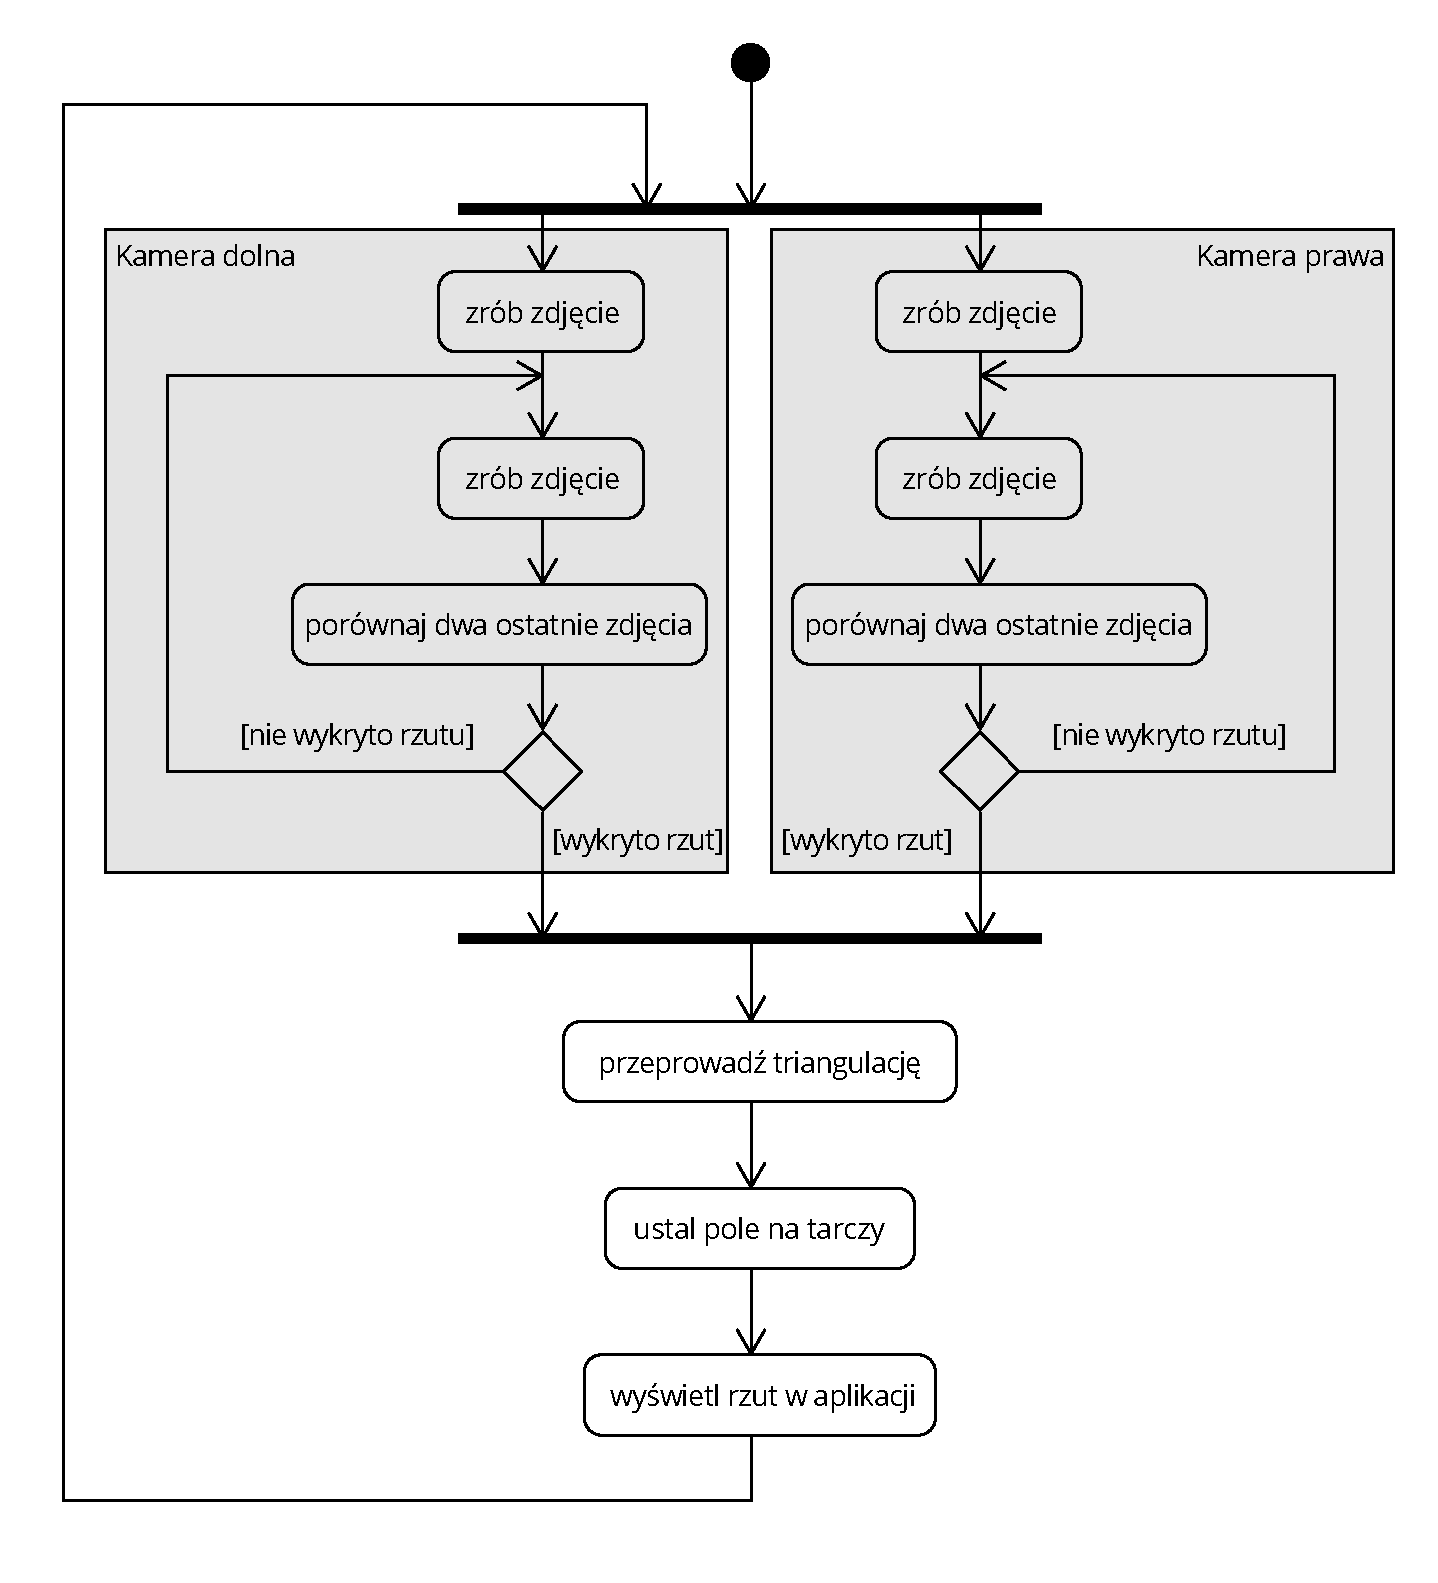
\includegraphics[width=\textwidth]{obrazki/activity.pdf}
\end{center}
\captionsource{{\color{dgray}Diagram aktywności}}{Opracowanie własne}
\label{activity}
\end{figure} 

\section{Diagramy sekwencji}
Diagram sekwencji (\ref{sequence}) pokazuje, w jaki sposób odbywa się komunikacja pomiędzy poszczególnymi komponentami. Jako pierwszy startuje program na \verb|Raspberry Pi 4|. Najpierw czeka on na połączenie z drugim minikomputerem, \verb|Pi Zero| oraz w osobnym wątku tworzy serwer dla aplikacji mobilnej. Gracz może wtedy włączyć aplikację, która natychmiastowo połączy się z tymże serwerem. W tym momencie gracz może zacząć wykonywanie rzutów. \verb|Pi 4| oraz \verb|Pi Zero| równolegle wykrywają rzut, lecz po wykryciu rzutu przez pierwszego z nich, czeka on na dane o położeniu piksela, nadchodzące z drugiego. Później, po przeprowadzeniu obliczeń, informacje o rzucie są przesyłane od serwera do aplikacji mobilnej. Możliwe jest podłączenie wielu klientów -- serwer posiada listę podłączonych użytkowników i wysyła informacje do każdego z nich. 
\begin{figure}[h!]
\begin{center}
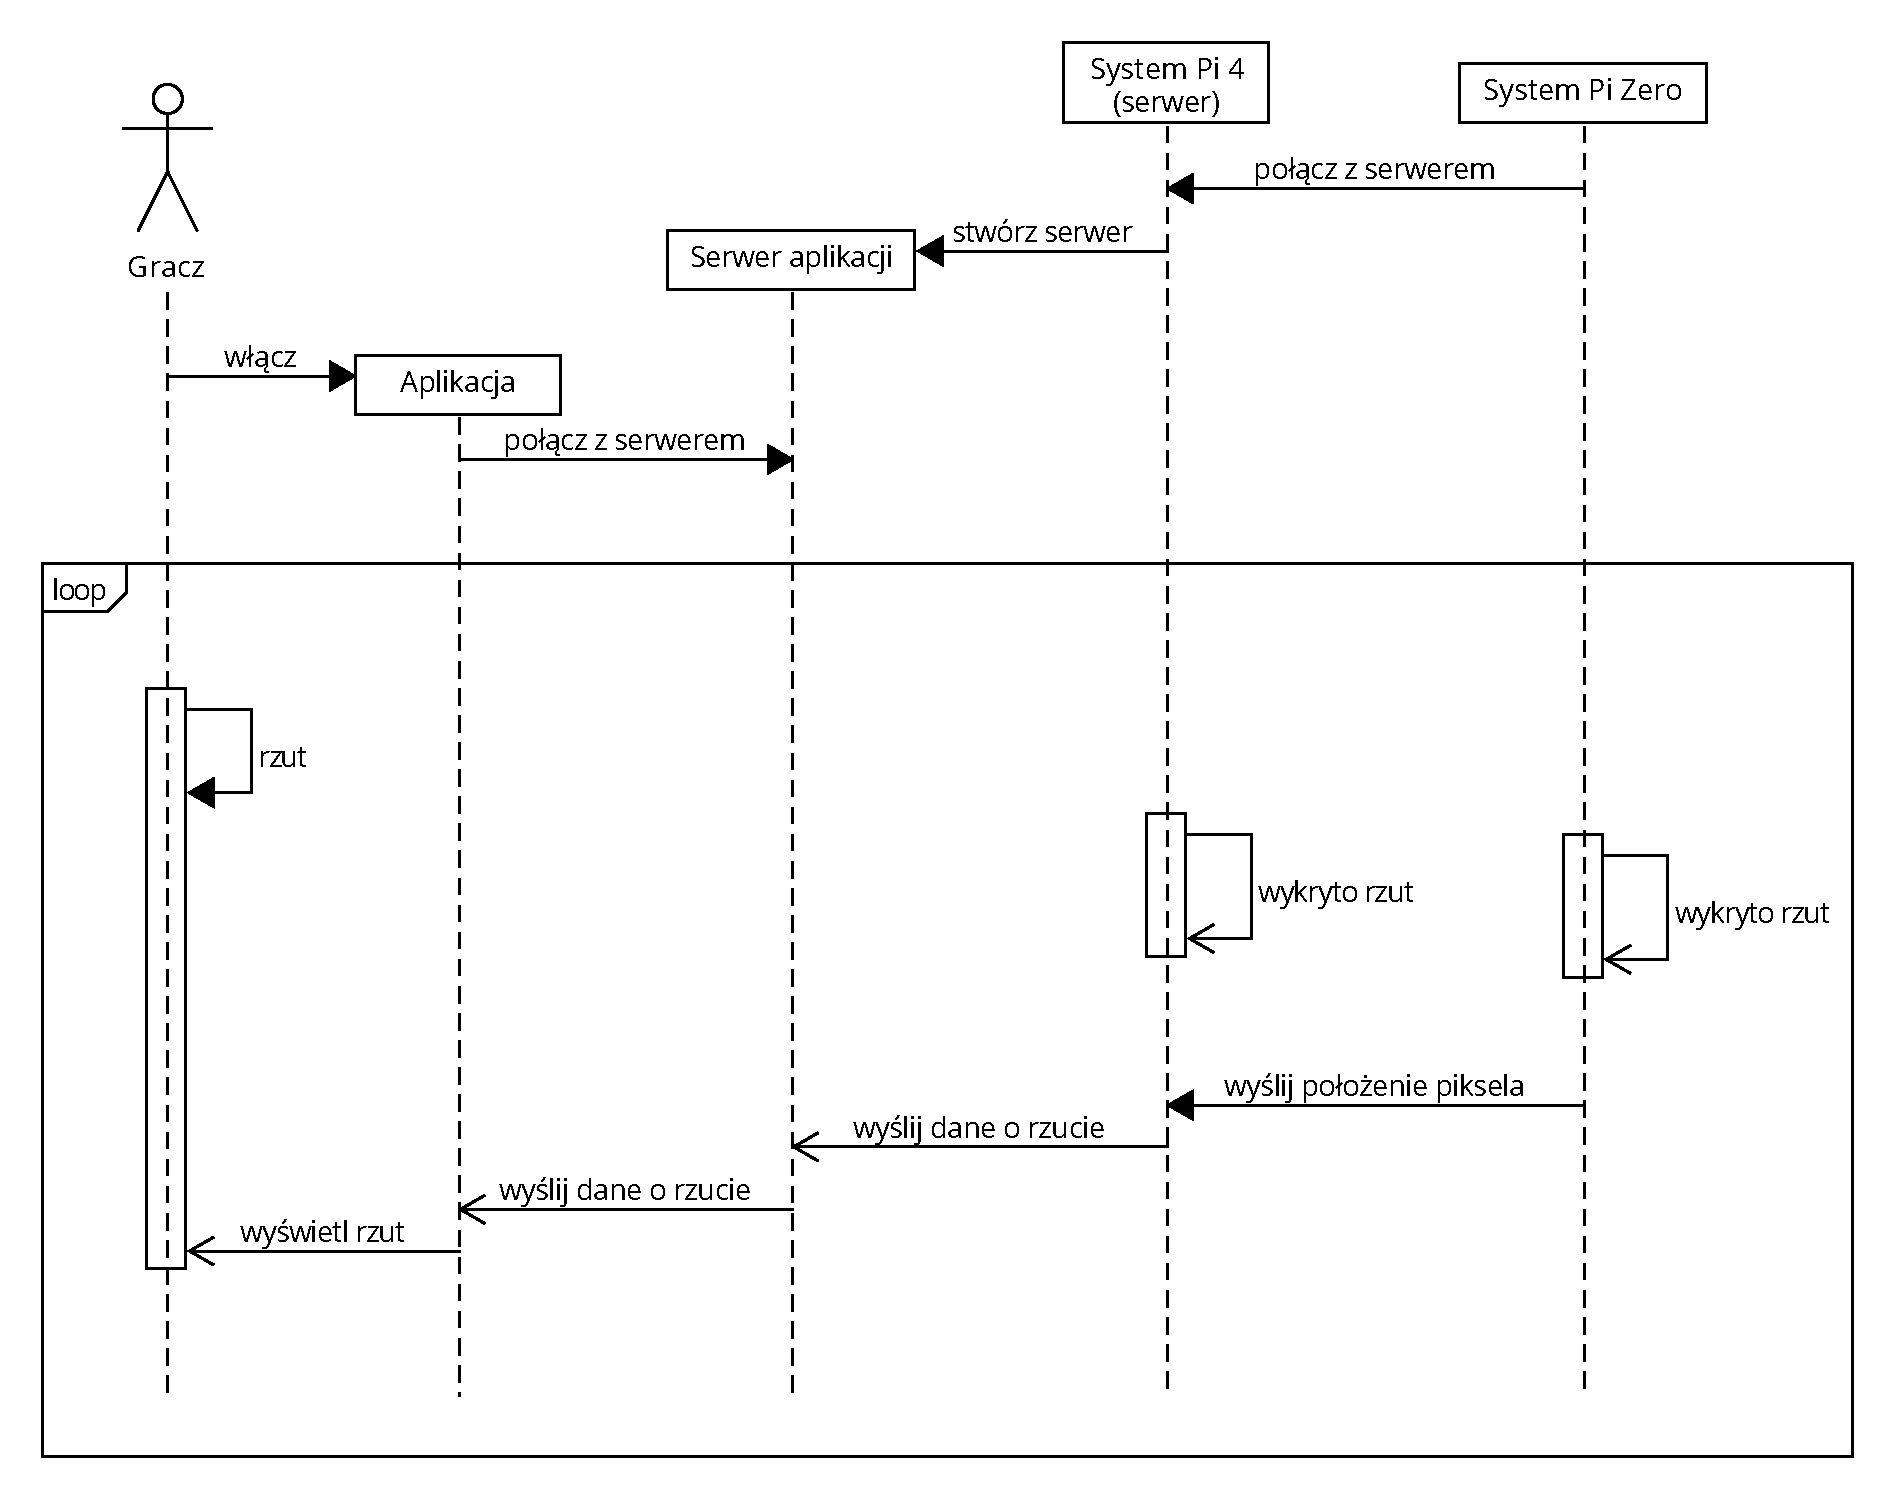
\includegraphics[width=\textwidth]{obrazki/sequence.pdf}
\end{center}
\captionsource{{\color{dgray}Diagram sekwencji}}{Opracowanie własne}
\label{sequence}
\end{figure}

\section{Opis protokołów}
W systemie do komunikacji używa się dwóch protokołów: TCP \cite{TCP} i WebSocket \cite{WebSocket}. Pierwszy z nich używany jest do wysłania informacji z \verb|Pi Zero| do \verb|Pi 4| w sposób binarny: 3 liczby całkowite (pozycja $x$, pozycja $y$ oraz liczba porządkowa rzutki), po 4 bajty na liczbę, w formacie \textit{big endian}. Drugi protokół stosuje się przy przekazaniu komunikatu o wyliczonej pozycji rzutki. Jego treść jest w formacie \verb|JSON| i została pokazana na listingu \ref{json}. 

\begin{listing}[h!]
\begin{minted}[frame=single,
               framesep=3mm,
               linenos=true,
               xleftmargin=21pt,
               tabsize=4]{js}
{     
    "x": 23.123516,
    "y" : 5.7825,
    "segment" : 20
}
\end{minted}
\caption{Przykładowy komunikat o wykrytej rzutce} 
\label{json}
\end{listing}

\section{Algorytm przetwarzania obrazu}
Podstawowym algorytmem, który nie został opisany w poprzednim rozdziale, jest proces przetwarzania obrazu. Zadaniem, które należy wykonać za pomocą metod związanych z tą dziedziną, jest odjęcie tła (ang. \textit{background substraction}). Polega ono na wyodrębnieniu elementów pojawiających się na pierwszym planie, na podstawie następujących po sobie zdjęć. W prezentowanym systemie użyte zostało w celu wykrycia rzutu, a następnie ustalenia samej pozycji rzutki na zdjęciu. W ogólności jest to zadanie trudne, ze względu na możliwe zmiany tła, spowodowane m.in. minimalnym ruchem lub zmianą warunków oświetlenia. Podejść do jego rozwiązania jest wiele \cite{LearningOpenCV}, jednak w niniejszej pracy, z powodu niewielkiej liczby tego typu czynników, zastosowano jedno z najprostszych - odejmowanie od siebie dwóch kolejnych klatek.

Każda z kamer, co pewien krótki czas, wykonuje zdjęcie. Następnie, dwa ostatnie zdjęcia z danej kamery, są od siebie odejmowane. Dzięki reprezentacji macierzowej, działanie to odbywa się zgodnie z zasadami bezwzględnego odejmowania macierzy. Jego wynikiem jest nowe zdjęcie, w której piksele niezmienione w czasie pomiędzy wykonaniem klatek powinny być bliskie wartości 0 (piksel czarny), zaś te reprezentujące pojawienie się nowego obiektu -- wyraźnie większe od zera. Aby zmniejszyć występujące szumy oraz przekształcić obraz na binarny (czarno-biały), stosuje się następnie funkcję progową (ang. \textit{threshold}), która wszystkie piksele o wartościach niższych od ustalonego progu zamienia na czarne, a wyższe -- na piksele białe. 

Tak przygotowane zdjęcie należy poddać wykrywaniu konturów. Konturem nazywa się zbiór punktów reprezentujących krzywą \cite{LearningOpenCV}. W przypadku problemu omawianego w pracy, celem jest wykrycie konturu wokół rzutki, która pojawiła się na ostatnio wykonanym zdjęciu. % TODO: opisz findContours()
Algorytm wykrywania konturów jest dość skomplikowany, jego szczegóły można znaleźć w pracach Suzuki \cite{ContoursAlgorithm}. Po uzyskaniu listy konturów wybierany jest największy z nich (pod względem powierzchni, którą wyznacza), a następny poddany analizie, czy jest to kontur rzutki. Należy wyznaczyć charakterystyczne cechy lotki na zdjęciu, opierając się na empirycznych danych pochodzących z testów. W obecnej implementacji kontur jest uznawany za kontur rzutki wtedy, gdy powierzchnia przez niego wyznaczona mieści się w określonych doświadczalnie granicach. Innymi sposobami jest na przykład sprawdzanie proporcji długości do szerokości w prostokącie okalającym kontur.  Jeśli nie wykryto żadnych konturów lub nie spełniają one warunków, uznaje się, że rzut nie wystąpił pomiędzy badanymi ujęciami.

Ostatnią fazą jest wybranie pojedynczego piksela, którego pozycja będzie reprezentować miejsce wbicia rzutki: jest to najniżej położony piksel konturu (znajdujący się najbliżej tarczy).